\chapter{Variant Hardness Prediction} \label{sec:subhrdnspred}
In this section, we attempt to determine how difficult variants from Algorithm~\ref{alg:ColSP} are for $\ColMod{N}{A}{8}$, where $A= \{1\}$, $\{5\}$, $\{7\}$, or $\{5,7\}$. We start by defining some measures, talk about the process how we ran experiments, and talk about the results, analyzing termination of the singleton set $A$ Collatz Variants 1, 5, and 7, and the combined 2-element variant of $\{5,7\}$ in separate sections. 
\section{Defining Measures} \label{subsec:algdefinemeasure} 
We define hardness off of the notion that odd numbers make the Collatz Conjecture harder, whereas even numbers make it easier. To more precisely define the measures, define the following numbers, given some input number $x$:
\begin{itemize}
    %\item $x_i$: the number $x$ turns into after $i$ steps of the Collatz Mapping have been applied.
    \item $f(x)$: The total number of steps in the sequence for $x$ before it converges to 1.
    \item $f_\text{odd}(x)$: Number of odd numbers visited in the sequence from $x$ to 1.\footnote{If one wanted to figure out the number of visited even numbers, then $f_\text{even}(x) = f(x) - f_\text{odd}(x)$} 
    \item $A$: The base avoidance set. Same as defined in Algorithm~\ref{alg:ColSP}. For the Collatz Variants we are exploring in this chapter, $A \subseteq \{1, 3, 5, 7\}$ and $A \ne \varnothing$.
    \item $g(x,A)$: The highest number of steps, for an input number $x$ that converges to 1, where $\forall a \in A$, $x_i \not\equiv a \Mod{8} \wedge x_i > 1$. This is counting the maximum number of steps before $\ColMod{N}{A}{8}$ would terminate for input number $N$.
    \item $g_\text{odd}(x,A):$ The number of odd numbers within the given $g(x,A)$
    \item Slice: a batch of numbers from some low number to some high number for a fixed $A$.
    \item $x_{\min}$: the lowest number of any slice.
    \item $x_{\max}$: the highest number of any slice.

    \item Record: any number $r$ in the range that has $g(r,A)$ higher than all numbers measured so far in the slice. More formally, any new record $r_\text{new}$ must have the properties compared to the current record $r_\text{current}$: $r_\text{new} > r_\text{current}$, and $g(r_\text{new},A) > g(r_\text{current},A)$ for a specific $A$. Note that we measure records off of total steps, \textit{not} total number of odd numbers.
      
\end{itemize}
Using these numbers, two different measures are defined, and the intuition behind why they were chosen is given as well: \par
\textbf{Hardness}: Defined to be $H(x,A) = \frac{g_\text{odd}(x,A)}{\log_2{x}}$. This assesses whether or not increasing the number of bits needed to represent the number $x$ changes the difficulty of determining a proof for Collatz Variants  1, 5, or 7, or $\{5,7\}$.  \par
Also define ``Classical Hardness'' as a comparison: $H_C(x) = \frac{f_\text{odd}(x)}{\log_2{x}}$. This computes $H$ with respect to the whole sequence, instead of trying to avoid specific numbers. Records for Classical Hardness occur when $r_\text{new} > r_\text{current}$ and $f(r_\text{new}) > f(r_\text{current})$. \par
\textbf{Percentage of Sequence}: Defined to be $P(x,A) = \frac{g_\text{odd}(x,A)}{f_\text{odd}(x)}$. This assesses what percentage of all odd numbers lie within the longest sequence for Collatz Variants 1, 5, 7, or $\{5,7\}$.

\section{Generating Results} \label{subsec:algcomp}
We wrote a program that computed Collatz Sequences using Java, and ran it on all odd numbers from 1 to 1 billion. The program has various modes which evolved over the lifetime of this project. In these modes, let $\mathcal{A}$ be a family of avoidance sets $A$ we wish to compute.
\begin{itemize}
    \item {\tt baseavoid} is the default option. This allows us to check all $A \in \mathcal{A}$ by running through all odd numbers from $x_{\min}$ (we usually use 1) to $x_{\max}$ (we usually use 1 billion), and determines the maximum number of steps we can run Algorithm~\ref{alg:ColSP} for each set $A \in \mathcal{A}$, or in other words, compute $g(x,A)$ for all odd $x$ in the range $x_{\min} \leq x \leq x_{\max}$. When it finishes, it prints out the longest sequence for each $A$.
    \item {\tt entirechain} just runs Algorithm~\ref{alg:ColR} for all odd $x$ in the range $x_{\min} \leq x \leq x_{\max}$, and prints out the longest sequence.
    \item {\tt untildecay} means that, for each odd number in between $x_{\min}$ and $x_{\max}$, we continue to run until we have a number lower than the original number. We return only the longest sequence of numbers that occurs until the resulting number is smaller than the initial number.
    \item {\tt updown} is a quite different mode. For each odd number $x$ such that $x_{\min}\leq x \leq x_{\max}$, determine two things. First, the number of steps it takes for $x$ to become some number $x_i$ such that $x_i < x$. Second, the number of steps it takes for another number $x_g$ to grow to $x$ if such an $x_g$ exists (no multiple of 3 can grow from a smaller number, for instance). The output prints out, for all odd numbers in the range, $x_i$, the number of steps it takes for $x$ to turn into $x_i$, and, if $x_g$ exists, the number $x_g$ and the number of steps it takes for $x_g$ to grow into $x$.
    \item {\tt avoidingmodgrowth} is a mode like baseavoid. However, it prints tables showing progressively growing records. This is the mode we used to generate the hardness results in this Thesis.
\end{itemize}
As mentioned, we used the {\tt avoidingmodgrowth} mode to generate the records defined in subsection~\ref{subsec:algcomp}. We run for sequences of odd numbers in multiple slices, usually 8, in order to take advantage of parallel computing via a distributed computing program called Condor that was made by The University of Wisconsin-Madison~\cite{Thain:2005:DCP:1064323.1064336}. We then combine the records of these 8 tables by hand using the defined record criterion. \par
We run sequences of numbers and have an option to avoid recomputing odd numbers already part of a prior Collatz Sequence, as these will never generate new records. However, this option can be disabled if we wish to compute extremely large numbers and slices, and are limited in our memory storage. \par
The program could have been rewritten to build off of previously used results, which should run faster, but this would have been difficult without many GBs of memory available and tight memory management on our program. So the space efficient approach was chosen for this project.\par
The code can be accessed via a public GitHub repository located at \url{https://github.com/mdenend/CollatzRewriteSystem}. A readme file is included that explains how to run the code and available options.
\section{Single Base Avoidance Analysis} \label{subsec:algsinglebase}
Our analysis for analyzing the termination of Collatz Variants 1, 5, and 7 is broken into three subsections: two exploring our defined computations, $H$ and $P$, and a third one analyzing interesting properties of sequence similarities that may provide insight to eventual proofs showing that these three Collatz Variants must terminate.
For exploring $H$ and $P$, we took all of the records for Collatz Variants 1, 5, and 7, and plotted the log of all records $r$ versus $H(x,A)$ and $P(x,A)$, respectively. We also added in Collatz Variant 3 as a reference for both of these measures as a control case.
\subsection{Hardness Function Results and Analysis} \label{subsubsec:algsinhardness}
Figure~\ref{fig:hvslog} shows the results of $H(x,A)$ versus the number of bits ($\log_2{x}$). Total steps for each mod number were also added in as well.\par
\begin{figure}
    \centering
    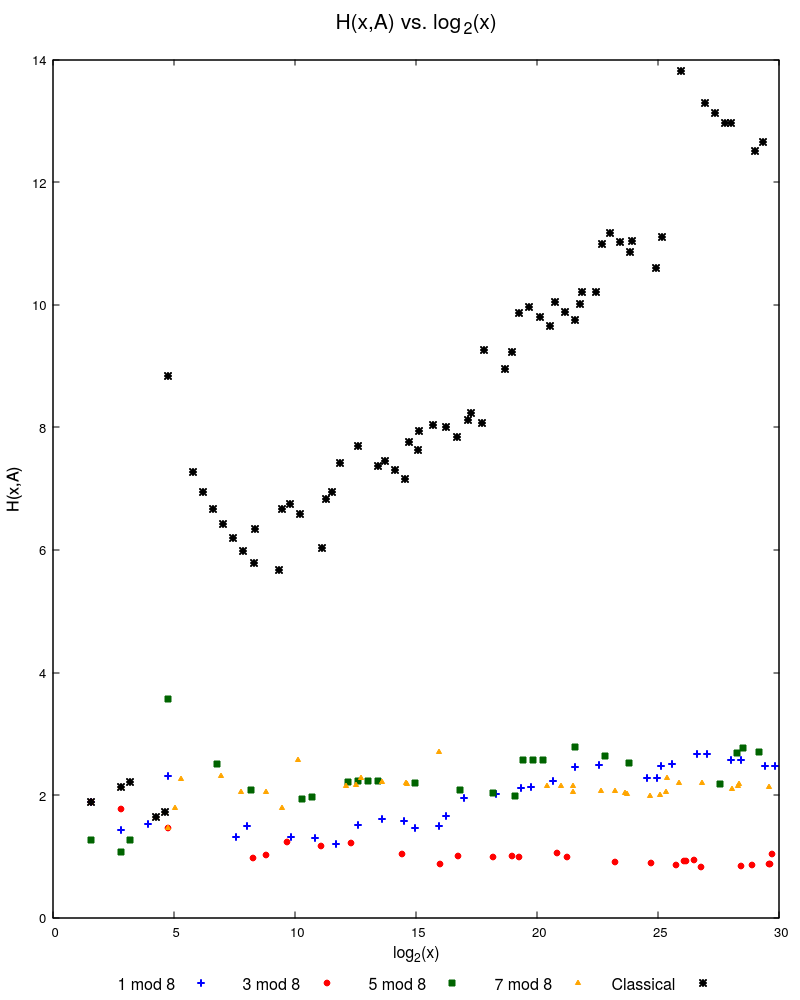
\includegraphics[scale=0.6]{ModAvoidanceAnalysisPics/H_vs_log.png}
    \caption{This graph visualizes how the $H$ values for Collatz Variants 1, 3, 5, and 7 compare to each other, and to classical hardness. The log of the record holding numbers, or number of bits needed, is the x-axis, and the hardness measure $H$ as defined in subsection~\ref{subsec:algdefinemeasure} is the y-axis.}
    \label{fig:hvslog}
\end{figure}
Comparing the three unproven Collatz Variants 1, 5, and 7 to the proven variant 3, the known variant is easier. The known variant actually slight decreases in hardness as the number of bits increases, meaning that there are fewer odd numbers per bit than the unproven variants. \par
Comparing the unknown variants to themselves, there is no consistent leader among the three as the number of bits increases. However, they all seem to be around within a hardness range of 1-3, with only a couple of exceptions. Variant 7 seems to remain in the same range with no definite increase or decrease, whereas variants 1 and 5 grow slightly from around 12 bits onward. The growth for both variants 1 and 5 may be because as numbers get larger, there are more opportunities to visit the $6 \rightarrow 7 \rightarrow 6$ cycle, which clearly adds odd numbers more quickly to the sequence than any other base 8 graph traversal. More experiments for higher numbers should be consider in order to determine whether any of these three unknown variants trend the same way as we add more bits into the computation.\par
Classical Hardness actually tends to grow linearly against the log scale, meaning that as the input number increases, the hardness increases logarithmically. This contrasts to all three unproven variants, which tend to stay between values of 1.5 and 3 for $H$ for numbers below 1 billion, meaning that figuring out proofs for the variants' termination is expected to be easier than proving the Collatz Conjecture.
\subsection{Percentage of Sequence Function Results and Analysis} \label{subsubsec:algsinpercentage}
 Figure~\ref{fig:pvslog} shows the results of $P(x,A)$ versus the number of bits. $P(x,A)$, as discussed earlier, is just calculating what percentage of the record sequence contributes to the overall decay of that sequence to 1. \par
\begin{figure}
    \centering
    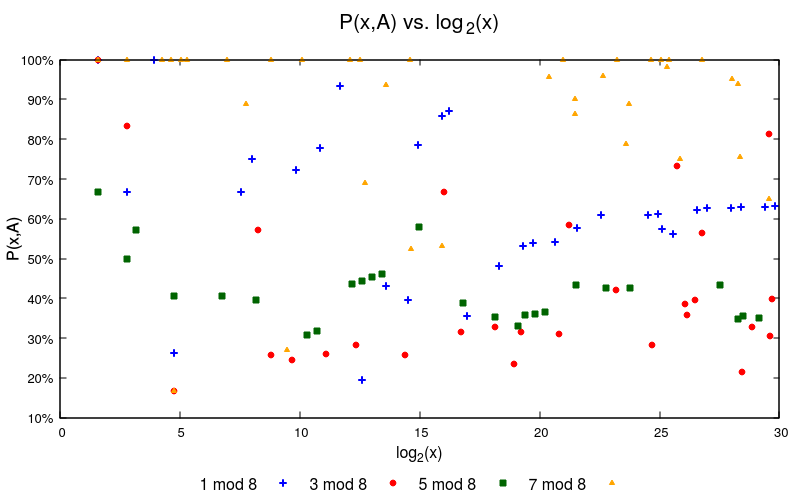
\includegraphics[scale=0.6]{ModAvoidanceAnalysisPics/P_vs_log.png}
    \caption{This graph visualizes how the $P$ values for Collatz Variants 1, 5, and 7 compare to each other. The log of the record holding numbers, or number of bits needed, is the x-axis, and the percentage measure $P$ as defined in subsection~\ref{subsec:algdefinemeasure} is the y-axis.}
    \label{fig:pvslog}
\end{figure}
Collatz Variant 7 comprises the highest percentage overall, with a couple of exceptions. Following Collatz Variant 7 causes the sequence to decline rapidly, since the $6 \rightarrow 7 \rightarrow 6$ cycle causes an input number to grow faster than any other cycle in the base 8 graph. Almost all of the records for variant 7 terminate at 1 instead of actually reaching a number that is $7 \Mod{8}$. \par
Variant 5 tends to have a low percentage, and appears to be the least erratic of all four variants. Variant 5 avoids the 0 self-cycle, which causes many divisions by 2. Numbers having a long sequence that prevent termination of variant 5 tend to have a very large number when they finally reach a number that is $5 \Mod{8}$, meaning that often, many more steps in the $3x+1$ mapping must be taken before these numbers converge to 1. \par
Variant 1 is interesting, because as the input numbers grow larger, the line changes from erratic behavior to a more steady percentage between approximately 50\% and 60\% at around 20 bits. This is likely a consequence of the sequence similarity that is seen in larger record for variant 1, which will be analyzed in subsubsection~\ref{subsubsec:algseqsim}. Further, as mentioned in the cycle analysis in subsection~\ref{subsubsec:cycleanalysis}, the $4 \rightarrow 6 \rightarrow 3 \rightarrow 2 \rightarrow 5 \rightarrow 0 \rightarrow \ldots \rightarrow 4$ cycle combined with the  $6 \rightarrow 7 \rightarrow 6$ cycle which avoidings node 1 causes a clash between the decay of the 0 self-cycle and the growth of the $6 \rightarrow 7 \rightarrow 6$ cycle, which may explain some of the erratic behavior for variant 1, aside from the small part with chain similarity. \par
Variant 3 tends toward the lowest percentage of all odd numbers, even lower than variant 5, but also has erratic behavior. This could be explained by the fact that avoiding termination of variant 3 causes the sequence to follow some combination of the $6 \rightarrow 7 \rightarrow 6$ cycle, the $4 \rightarrow 2 \rightarrow 1 \rightarrow 4$ cycle, or the $4 \rightarrow 2 \rightarrow 5 \rightarrow 0  \rightarrow \ldots \rightarrow 4$ cycle with some number of $0$ self-cycles. The first cycle causes growth, whereas all three other cycles cause decay. If the growth cycle is followed, the number gets larger, likely reducing the percentage of odd numbers making up long chains avoiding termination of variant 3, whereas the decay cycles cause the number to shrink, tending the percentages to be higher. This may explain why variant 3 causes widely different percentages.
\subsection{Sequence similarity analysis} \label{subsubsec:algseqsim}
We analyzed the sequences of the records for Collatz Variants 1, 5, and 7 as well to see if we could find any similarities:
\begin{itemize}
    \item Variant 1: There are two groups of records that were particularly interesting: Those from 325,791 to 32,505,681 (call this group $S$), and those from 35,651,835 to 949,643,331 (call this group $T$). Group $S$ numbers all terminated at number 161, and group $T$ numbers all terminated at number 35,369. These sequences all matched \textit{number-by-number} at least one other sequence starting at most 8 steps from the beginning. This is a striking similarity meaning that records for variant 1 might be predictably related to groups $S$ or $T$, or perhaps to other groups.
    \item Variant 7: All record sequences, except for input number 27, terminated at 1. While there was some similarity between sequences (all numbers $\geq 62079$ had the same last 41 numbers), there were many different paths taken from the input, so not as many patterns here.
    \item Variant 5: This had few matches and was the most changing of the records, so chain similarity appears not to have did not have as much to do with the low variance that $P$ has for variant 5.
\end{itemize}
\section{Paired Base Avoidance Analysis} \label{subsec:algpairedbase}
Since termination of Collatz Variants 1, 5, and 7 appear to be difficult to prove, we also analyzed two element combinations of them. The termination of two such variants were already proved in subsection~\ref{subsubsec:base8subprob}: $\{1,5\}$ and $\{1,7\}$. However, termination of variant $\{5,7\}$ is unknown. This section will analyze what happens to $H(x,A)$ and $P(x,A)$ where $A=\{1,5\}$, $\{1,7\}$, and $\{5,7\}$.
\subsection{Hardness Function Results and Analysis} \label{subsubsec:algmulhardness}
\begin{figure}
    \centering
    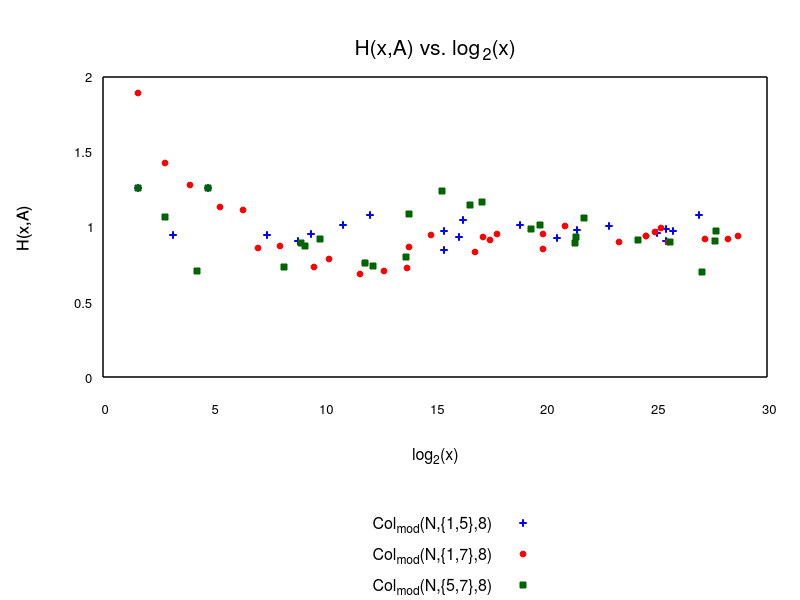
\includegraphics[scale=0.6]{ModAvoidanceAnalysisPics/H_vs_log_multi_base.png}
    \caption{This graph visualizes the $H$ measure for the three Collatz Variants $\{1,5\}$, $\{1,7\}$, and $\{5,7\}$. The log of the record holding numbers, or number of bits needed, is the x-axis, and the hardness measure $H$ as defined in subsection~\ref{subsec:algdefinemeasure} is the y-axis. Classical Hardness was omitted from this graph to eliminate distortion.}
    \label{fig:h_multivslog}
\end{figure}
Figure~\ref{fig:h_multivslog} shows the results of $H(x,A)$ versus $\log_2{x}$. These results were quite surprising. At first thought, it would have appeared that the unproven variant $\{5, 7\}$ should be the hardest to determine, compared to the two variants we have proofs for. But both variants $\{1, 5\}$ and $\{1, 7\}$  had alike predictive hardness to $\{5, 7\}$! These numbers suggest that a proof for determining why variant $\{5, 7\}$ must terminate is either easier than we anticipated, or our hardness measures are not very good. However, given the fact that variant 3 for the single base cases is clearly easier than variants 1, 5, and 7, we have reason to believe this measure should be good. Further investigation needs to be considered.
\subsection{Percentage of Sequence Function Results and Analysis} \label{subsubsec:algmulpercentage}
\begin{figure}
    \centering
    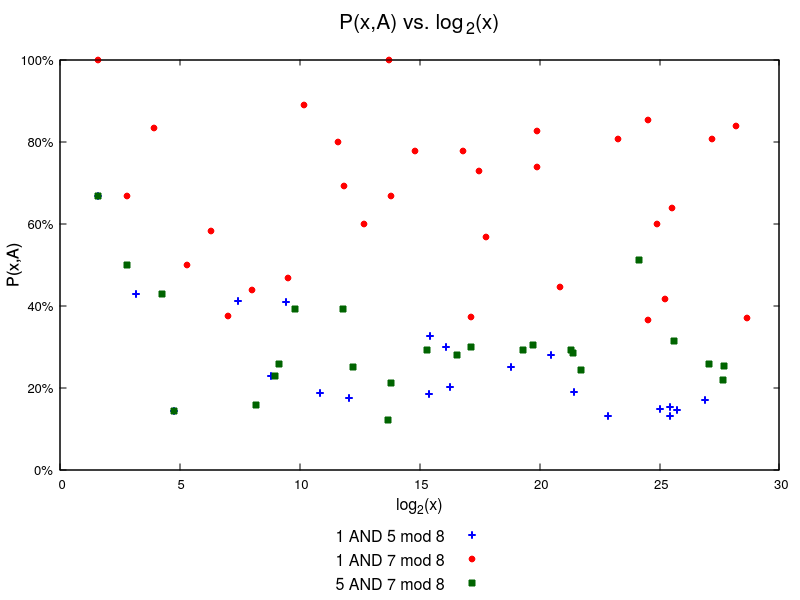
\includegraphics[scale=0.6]{ModAvoidanceAnalysisPics/P_vs_log_multi_base.png}
    \caption{This graph visualizes the $P$ measure for variants $\{1,5\}$, $\{1,7\}$, and $\{5,7\}$. The log of the record holding numbers, or number of bits needed, is the x-axis, and the hardness measure $P$ as defined in subsection~\ref{subsec:algdefinemeasure} is the y-axis.}
    \label{fig:p_multi_vslog}
\end{figure}
Figure~\ref{fig:p_multi_vslog} shows the results of $P(x,A)$ versus $\log_2{x}$. The variant $\{1,7\}$ makes up the highest percentage of the sequence compared to the other two cases, because avoiding both the $6 \rightarrow 7 \rightarrow 6$ and the $4 \rightarrow 6 \rightarrow 3 \rightarrow 2 \rightarrow 1 \rightarrow 4$ cycles only allows for the sequence to go through the $4  \rightarrow 2 \rightarrow 5 \rightarrow 0 \rightarrow \ldots \rightarrow 4$ cycle, causing fast decay, like with variant 7. \par
Both variants $\{1,5\}$ and $\{5,7\}$ are much closer to each other in percentage of total sequence, although as the numbers grow past 17 bits in size, variant $\{5,7\}$ comprises of the higher percentage of the sequence. A possible explanation is the fact that the $6 \rightarrow 7 \rightarrow 6$ cycle allowed in variant $\{1,5\}$ allows causes a number to grow larger than the $4 \rightarrow 6 \rightarrow 3 \rightarrow 2 \rightarrow 1$ cycle that variant $\{5,7\}$ allows. Also, since variant $\{1,5\}$ allows for larger numbers, and larger numbers generally (but not always) take more steps to decline, allowing for more growth should mean that the long sequence avoiding termination of variant $\{1,5\}$ comprises a lower percentage of all odd numbers.
